\begin{frame}
\frametitle{Experiments - Paired Image Translation}
\framesubtitle{Baselines}
Training details:
\begin{itemize}
    \item 330MB of trainable parameters for unpaired models(LoRA weights, zero-conv layer, first conv layer of U-Net)
    \item Adam Optimizer with learning rate: 1e-6, batch size:8, $\lambda _{\text{idt}} = 1$, $\lambda _{\text{GAN}} = 0.5$
\end{itemize}
Datasets:
\begin{table}
    \centering
    \begin{tabular}{|c|c|c|c|}
        Task & Images Source & Images Target & Dataset \\
        \hline
        Horse $\leftrightarrow$ Zebra & 939 & 1177 & ImageNet \cite{5206848}\\
        Winter $\leftrightarrow$ Summer & 854 & 1273 & Flickr \cite{zhu2020unpaired} \\
        Day $\leftrightarrow$ Night & Day subset & Night subset & BDD100k \cite{yu2020bdd100k}\\
        Clear $\leftrightarrow$ Foggy & 12454 & 572 from & BDD100k and DENSE \cite{bijelic2020seeing}
    \end{tabular}       
\end{table}
\end{frame}

\begin{frame}
    \frametitle{Experiments - Paired Image Translation}
    \framesubtitle{Baselines}
    Evaluation Protocol:
    \begin{itemize}
        \item match data distribution of target domain $\rightarrow$ FID \cite{heusel2018gans}
        \item preserve input image structure in translated output $\rightarrow$ DINO \cite{tumanyan2022splicing}
        \item Inference runtime using a single NVIDIA RTX A6000 GPU
        \item human preceptual study
    \end{itemize}
    
    
\end{frame}

% ---------- Comparison to Unpaired Methods ----------
\begin{frame}
    \frametitle{Experiments - Paired Image Translation}
    \framesubtitle{Comparison to Unpaired Methods}
    \begin{figure}
        \centering
        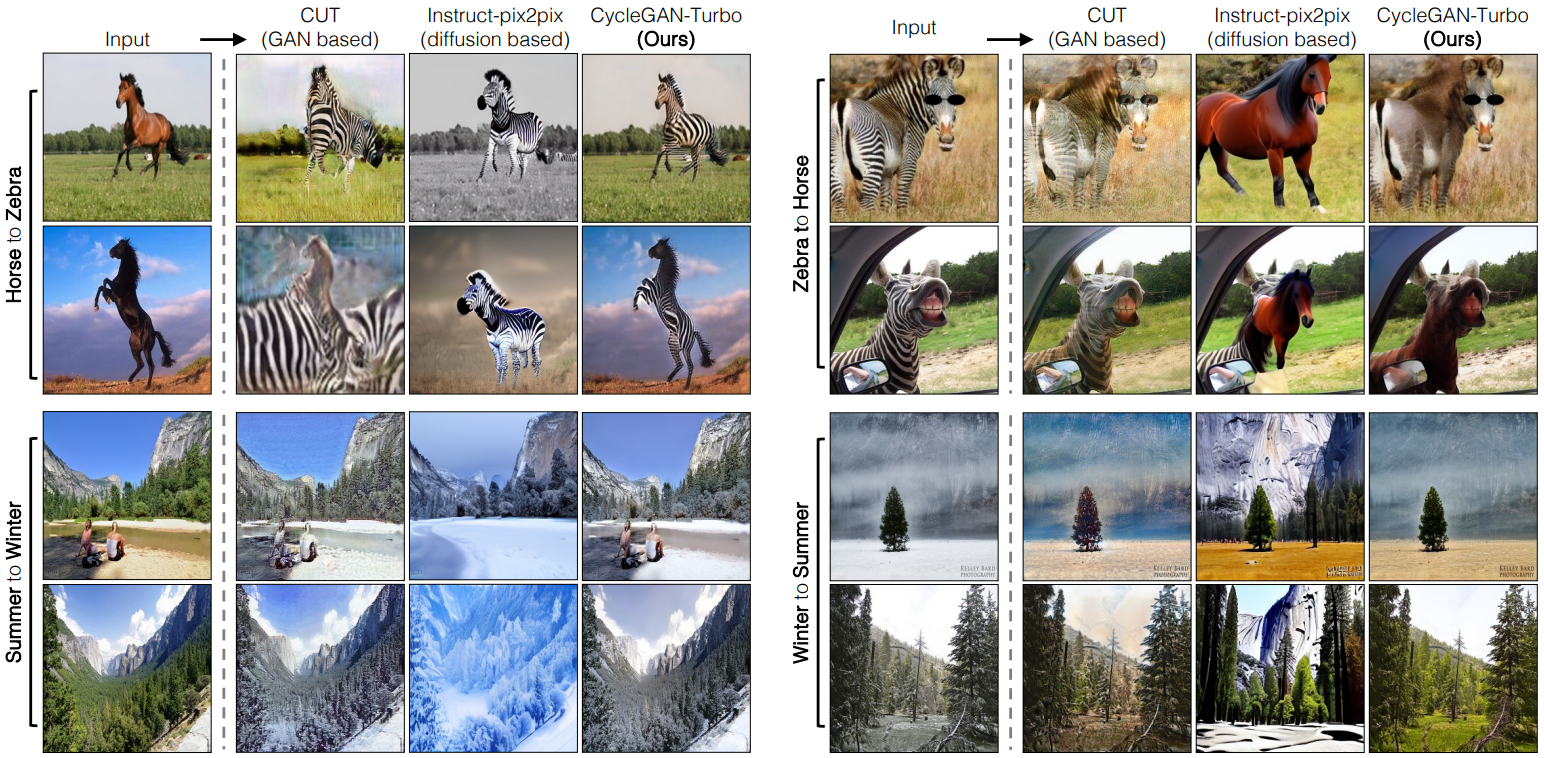
\includegraphics[width=0.85\linewidth]{images/horse_zebra.png}
        
    \end{figure}
\end{frame}

\begin{frame}
    \frametitle{Experiments - Paired Image Translation}
    \framesubtitle{Comparison to Unpaired Methods}
    \begin{figure}
        \centering
        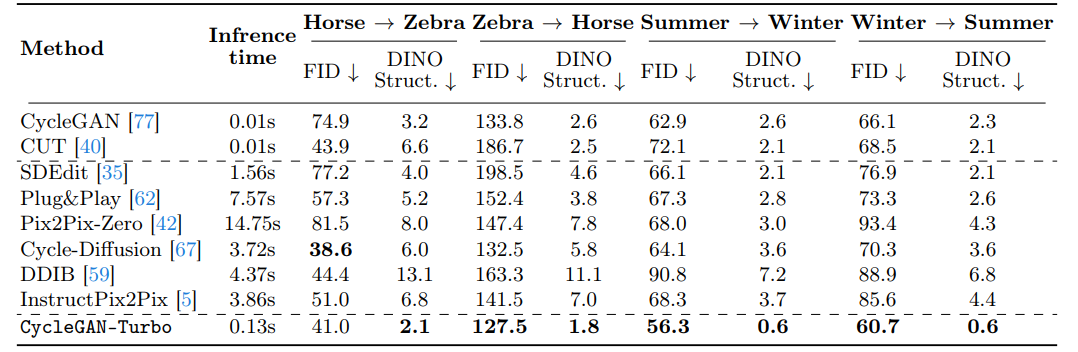
\includegraphics[width=1\linewidth]{images/horse_zebra_table.png}
        
    \end{figure}
\end{frame}

\begin{frame}
    \frametitle{Experiments - Paired Image Translation}
    \framesubtitle{Comparison to Unpaired Methods}
    \scriptsize\centering\begin{tabular}{c c c c c c c c c c}
        \Xhline{2\arrayrulewidth}
        \multirow{2}{*}{\textbf{Method}} & \multirow{2}{*}{\textbf{\makecell{Inference \\ time}}}  & \multicolumn{2}{c}{\textbf{Horse $\rightarrow$ Zebra}} & \multicolumn{2}{c}{\textbf{Zebra $\rightarrow$ Horse}} & \multicolumn{2}{c}{\textbf{Summer $\rightarrow$ Winter}} & \multicolumn{2}{c}{\textbf{Winter $\rightarrow$ Summer}}\\
        \cline{3-4} \cline{5-6} \cline{7-8} \cline{9-10}
        & & FID $\downarrow$ & \makecell{DINO \\ Struct. $\downarrow$} & FID $\downarrow$ & \makecell{DINO \\ Struct. $\downarrow$} & FID $\downarrow$ & \makecell{DINO \\ Struct. $\downarrow$} & FID $\downarrow$ & \makecell{DINO \\ Struct. $\downarrow$} \\
        \cline{1-10}
        CycleGAN \cite{zhu2020unpaired} & 0.01s & 74.9 & 3.2 & 133.8 & 2.6 & 62.9 & 2.6 & 66.1 & 2.3\\ 
        CUT \cite{park2019semantic} & 0.01s & 43.9 & 6.6 & 196.7 & 2.5& 72.1& 2.1 & 68.5 & 2.1\\
        \cline{1-10}
        SDEdit \cite{meng2022sdedit} & 1.56s & 77.2 & 4.0 & 198.5 & 4.6 & 66.1 & 2.1 & 76.9 & 2.1 \\
        Plug-and-Play \cite{tumanyan2022plugandplay} & 7.57s & 57.3 & 5.2 & 152.4& 3.8 & 67.3 & 2.8 & 73.3 & 2.6\\
        Pix2Pix-Zero & 14.75s & 81.5 & 8.0 & 147.4 & 7.8 & 68.0 & 3.0 & 93.4 & 4.3 \\
        Cycle-Diffusion & 3.72s & \textbf{38.6} & 6.0 & 132.5 & 5.8 & 64.1 & 3.6 & 70.3 & 3.6 \\
        DDIB & 4.37s & 44.4 & 13.1 & 163.3 & 11.1 & 90.8 & 7.2 & 88.9 & 6.8\\
        InstructPix2Pix & 3.86s & 51.0 & 6.8 & 141.5 & 7.0 & 68.3 & 3.7 & 85.6 & 4.4\\
        \cline{1-10}
        \textbf{CycleGAN-Turbo} & 0.13s & 41.0 & \textbf{2.1} & \textbf{127.5} & \textbf{1.8} & \textbf{56.3} & \textbf{0.6} & \textbf{60.7} & \textbf{0.6}\\
        \Xhline{2\arrayrulewidth}
        \end{tabular}
\end{frame}

\begin{frame}
\frametitle{Experiments - Paired Image Translation}
\framesubtitle{Comparison to Unpaired Methods}
\begin{figure}
    \centering
    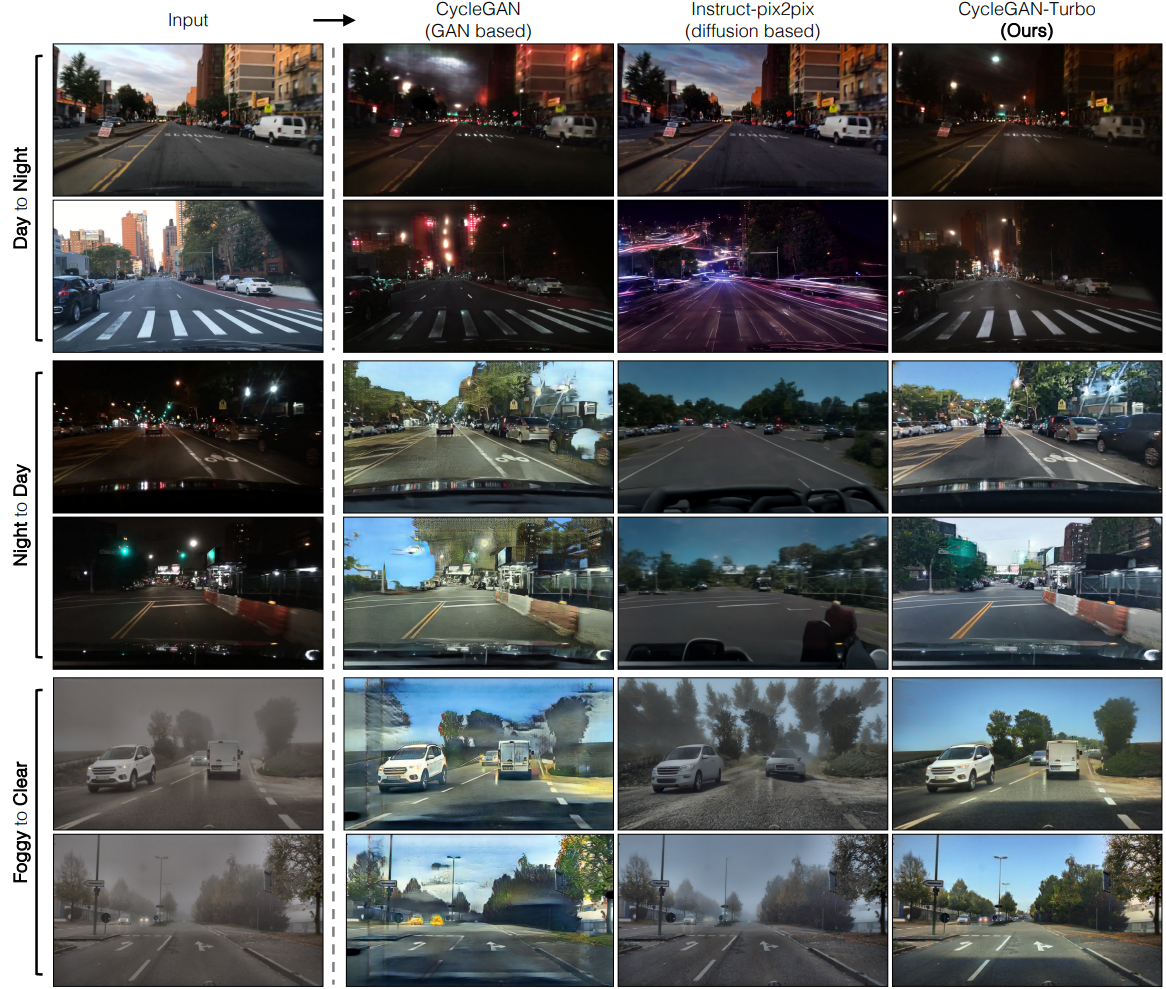
\includegraphics[width=0.5\linewidth]{images/day_night.png}
    
\end{figure}
\end{frame}

\begin{frame}
    \frametitle{Experiments - Paired Image Translation}
    \framesubtitle{Comparison to Unpaired Methods}
    \begin{figure}
        \centering
        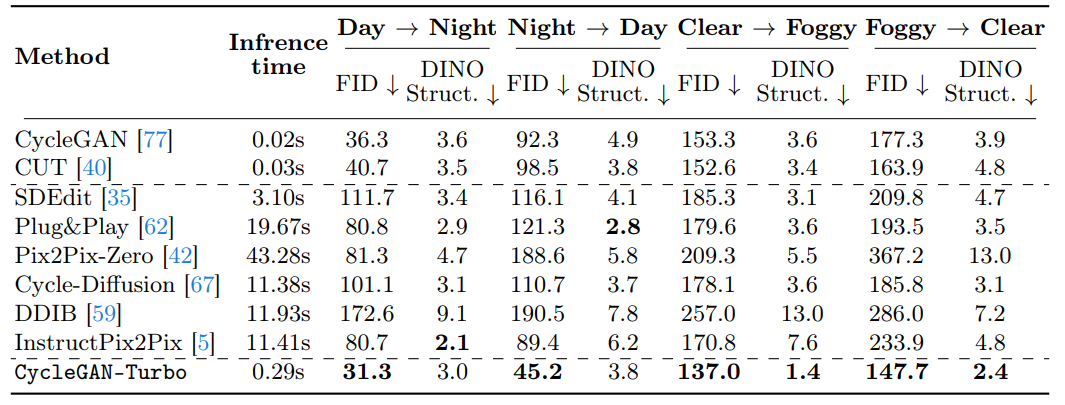
\includegraphics[width=1\linewidth]{images/day_night_table.png}
        
    \end{figure}
\end{frame}

\begin{frame}
    \frametitle{Experiments - Paired Image Translation}
    \framesubtitle{Comparison to Unpaired Methods}
    \begin{figure}
        \centering
        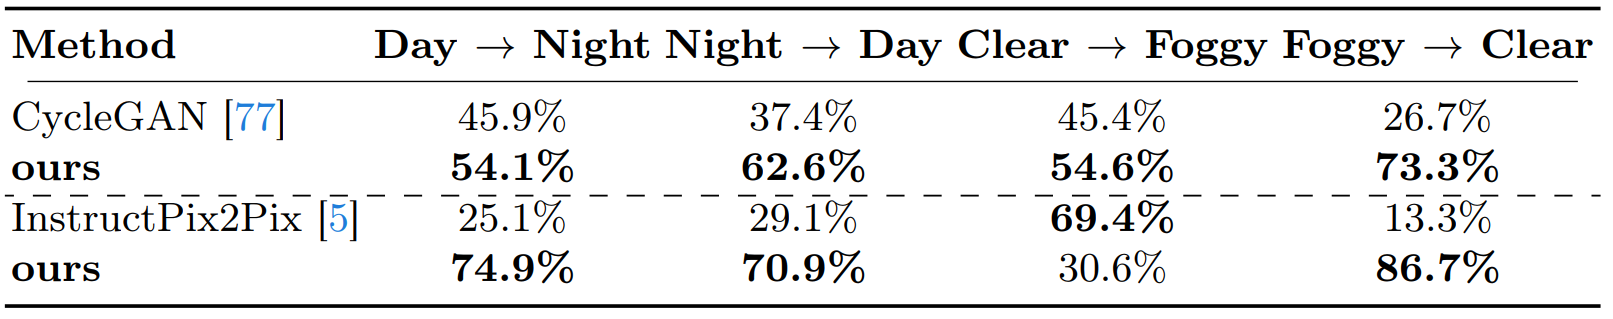
\includegraphics[width=1\linewidth]{images/human-pref.png}
        
    \end{figure}
\end{frame}


% ---------- Ablation Study ----------
\begin{frame}
\frametitle{Experiments - Paired Image Translation}
\framesubtitle{Ablation Study}
\begin{figure}
    \centering
    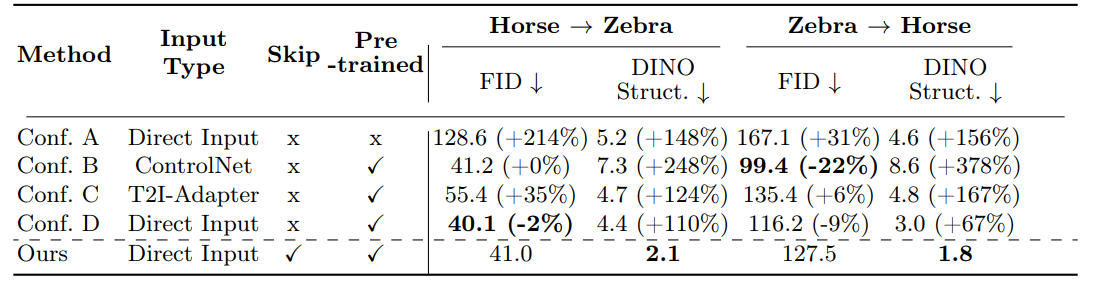
\includegraphics[width=1\linewidth]{images/ablation_horse_zebra.png}
    
\end{figure}
\end{frame}

\begin{frame}
    \frametitle{Experiments - Paired Image Translation}
    \framesubtitle{Ablation Study}
    \begin{figure}
        \centering
        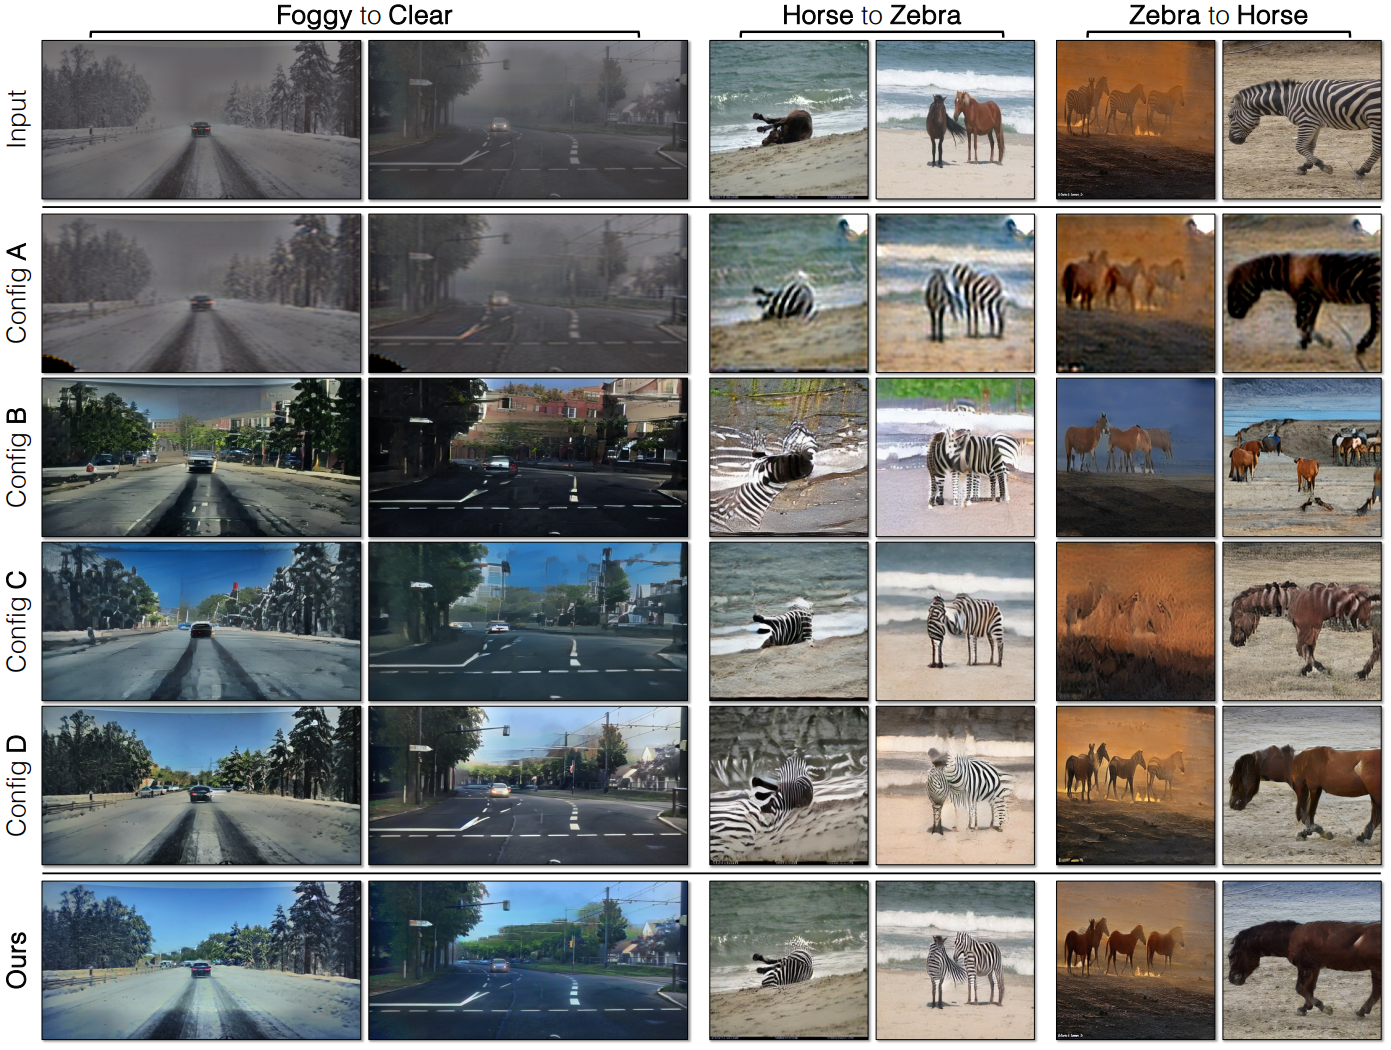
\includegraphics[width=0.55\linewidth]{images/ablation_images.png}
        
    \end{figure}
    \end{frame}
% ---------- Extensions ----------
\begin{frame}
\frametitle{Experiments - Unpaired Image Translation}
\framesubtitle{Training Details}
\begin{block}{Loss function}
    \begin{align}
        \arg \underset{G}{\min} \mathcal{L}_{\text{rec}} + \lambda _{\text{clip}} \mathcal{L}_{\text{CLIP}} + \lambda_{\text{GAN}}\mathcal{L}_{\text{GAN}}
    \end{align}
\end{block}
with $\mathcal{L}_{\text{rec}}$ = L2-Norm + LPIPS, $\lambda_{\text{clip}} = 4$ and $\lambda_{\text{GAN}} = 0.4$
\end{frame}

\begin{frame}
    \frametitle{Experiments - Unpaired Image Translation}
    \framesubtitle{Training Details}
        Edge-to-Image:
        \begin{itemize}
            \item Canny Edge Detector with random threshold
            \item Adam Optimizer with learning rate: 1e-5, batch size: 40, Steps: 7500
        \end{itemize}
        Sketch-to-Image:
        \begin{itemize}
            \item Synthetic sketches with multiple augmentations
            \item Initialized with Edge-to-Image model and fine-tuned for 5000 steps with same Optimizer
        \end{itemize}
\end{frame}

\begin{frame}
    \frametitle{Experiments - Unpaired Image Translation}
    \framesubtitle{Comparison to Unpaired Methods}
    \begin{figure}
        \centering
        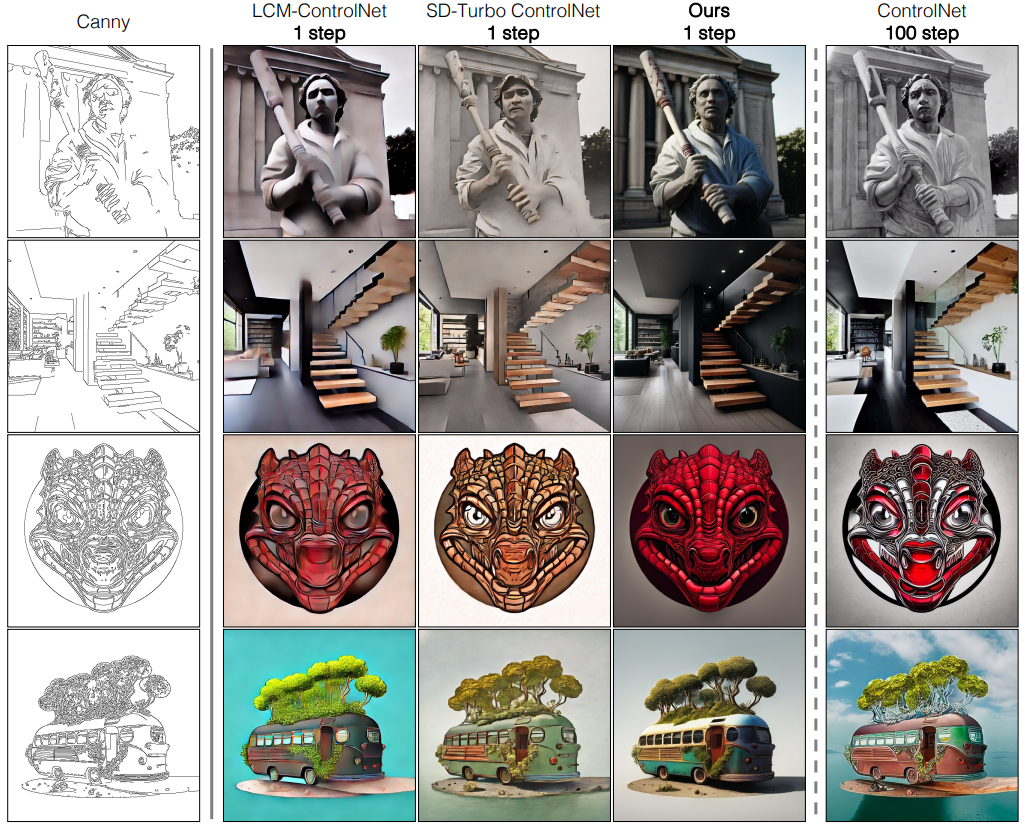
\includegraphics[width=0.5\linewidth]{images/unpaired_comp1.png}
        
    \end{figure}
\end{frame}

\begin{frame}
    \frametitle{Experiments - Unpaired Image Translation}
    \framesubtitle{Comparison to Unpaired Methods}
    \begin{figure}
        \centering
        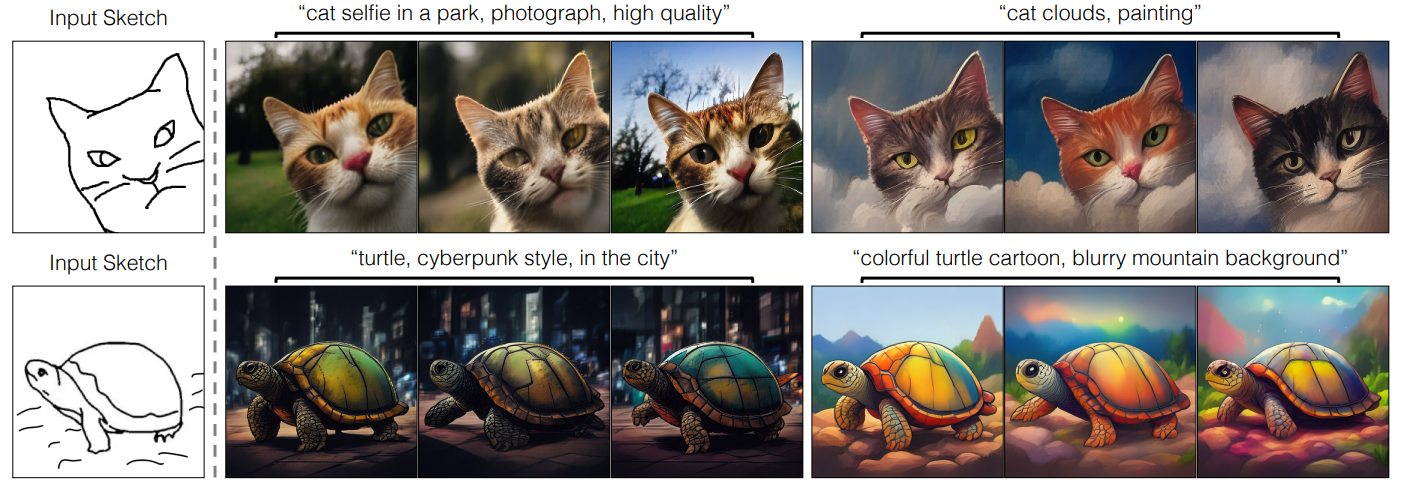
\includegraphics[width=1\linewidth]{images/unpaired_comp2.png}
            
    \end{figure}
\end{frame}
